\section{Image Deblurring}

\begin{bigidea}
Matrix multiplication by Toeplitz matrices perform blurring operations on a matrix $A_cXA_r^T = B$. Introducing some error $E$, we need to consider the truncated pseudoinverses $(A_c)^+_k$ and $(A_r)^+_k$ to reduce inverted noise.
\end{bigidea}

\begin{definition}
A {\bf Toeplitz matrix} \cite[p.34]{HNO} has constant values along the diagonals such as
$$
\begin{bmatrix}
p_3 & p_2 & p_1 & & \\
p_4 & p_3 & p_2 & p_1 & \\
p_5 & p_4 & p_3 & p_2 & p_1 \\
& p_5 & p_4 & p_3 & p_2 \\
& & p_5 & p_4 & p_3 \\
\end{bmatrix}
$$
\end{definition}

\begin{note}
Multiplying on the left by a Toeplitz matrix will spread (or ``blur") the values of a matrix $X$ vertically in the columns. For example, consider the Toeplitz matrix $A_c$ (where ``c" stands for ``columns") and image matrix $X$ and compute
$$
A_c X =
\begin{bmatrix}
1 & 1 & 0 & 0 & 0 \\
1 & 1 & 1 & 0 & 0 \\
0 & 1 & 1 & 1 & 0 \\
0 & 0 & 1 & 1 & 1 \\
0 & 0 & 0 & 1 & 1
\end{bmatrix}
\begin{bmatrix}
0 & 0 & 0 & 0 & 0 \\
0 & 1 & 1 & 1 & 0 \\
0 & 1 & 1 & 1 & 0 \\
0 & 1 & 1 & 1 & 0 \\
0 & 0 & 0 & 0 & 0
\end{bmatrix}
=
\begin{bmatrix}
0 & 1 & 1 & 1 & 0 \\
0 & 2 & 2 & 2 & 0 \\
0 & 3 & 3 & 3 & 0 \\
0 & 2 & 2 & 2 & 0 \\
0 & 1 & 1 & 1 & 0
\end{bmatrix}
$$
Similarly, multiplying on the right by a Toeplitz matrix will spread the values of a matrix $X$ horizontally in the rows. For example, consider the Toeplitz matrix $A_r$ (where ``r" stands for ``rows") and image matrix $X$ and compute
$$
X A_r^T =
\begin{bmatrix}
0 & 0 & 0 & 0 & 0 \\
0 & 1 & 1 & 1 & 0 \\
0 & 1 & 1 & 1 & 0 \\
0 & 1 & 1 & 1 & 0 \\
0 & 0 & 0 & 0 & 0
\end{bmatrix}
\begin{bmatrix}
1 & 0.5 & 0 & 0 & 0 \\
0.5 & 1 & 0.5 & 0 & 0 \\
0 & 0.5 & 1 & 0.5 & 0 \\
0 & 0 & 0.5 & 1 & 0.5 \\
0 & 0 & 0 & 0.5 & 1
\end{bmatrix}^T
=
\begin{bmatrix}
0.0 & 0.0 & 0.0 & 0.0 & 0.0 \\
0.5 & 1.5 & 2.0 & 1.5 & 0.5 \\
0.5 & 1.5 & 2.0 & 1.5 & 0.5 \\
0.5 & 1.5 & 2.0 & 1.5 & 0.5 \\
0.0 & 0.0 & 0.0 & 0.0 & 0.0
\end{bmatrix}
$$
By convention, we take the transpose of the matrix $A_r$ when we use it to blur the rows.
\end{note}

\begin{example}
Consider the symmetric Toeplitz matrix $A$ where the first row is given by
$$
\begin{bmatrix}
1.00 & 0.75 & 0.50 & 0.25 & 0.00 & \cdots & 0.00
\end{bmatrix}
$$
We can visualize the matrix $A$
\begin{center}
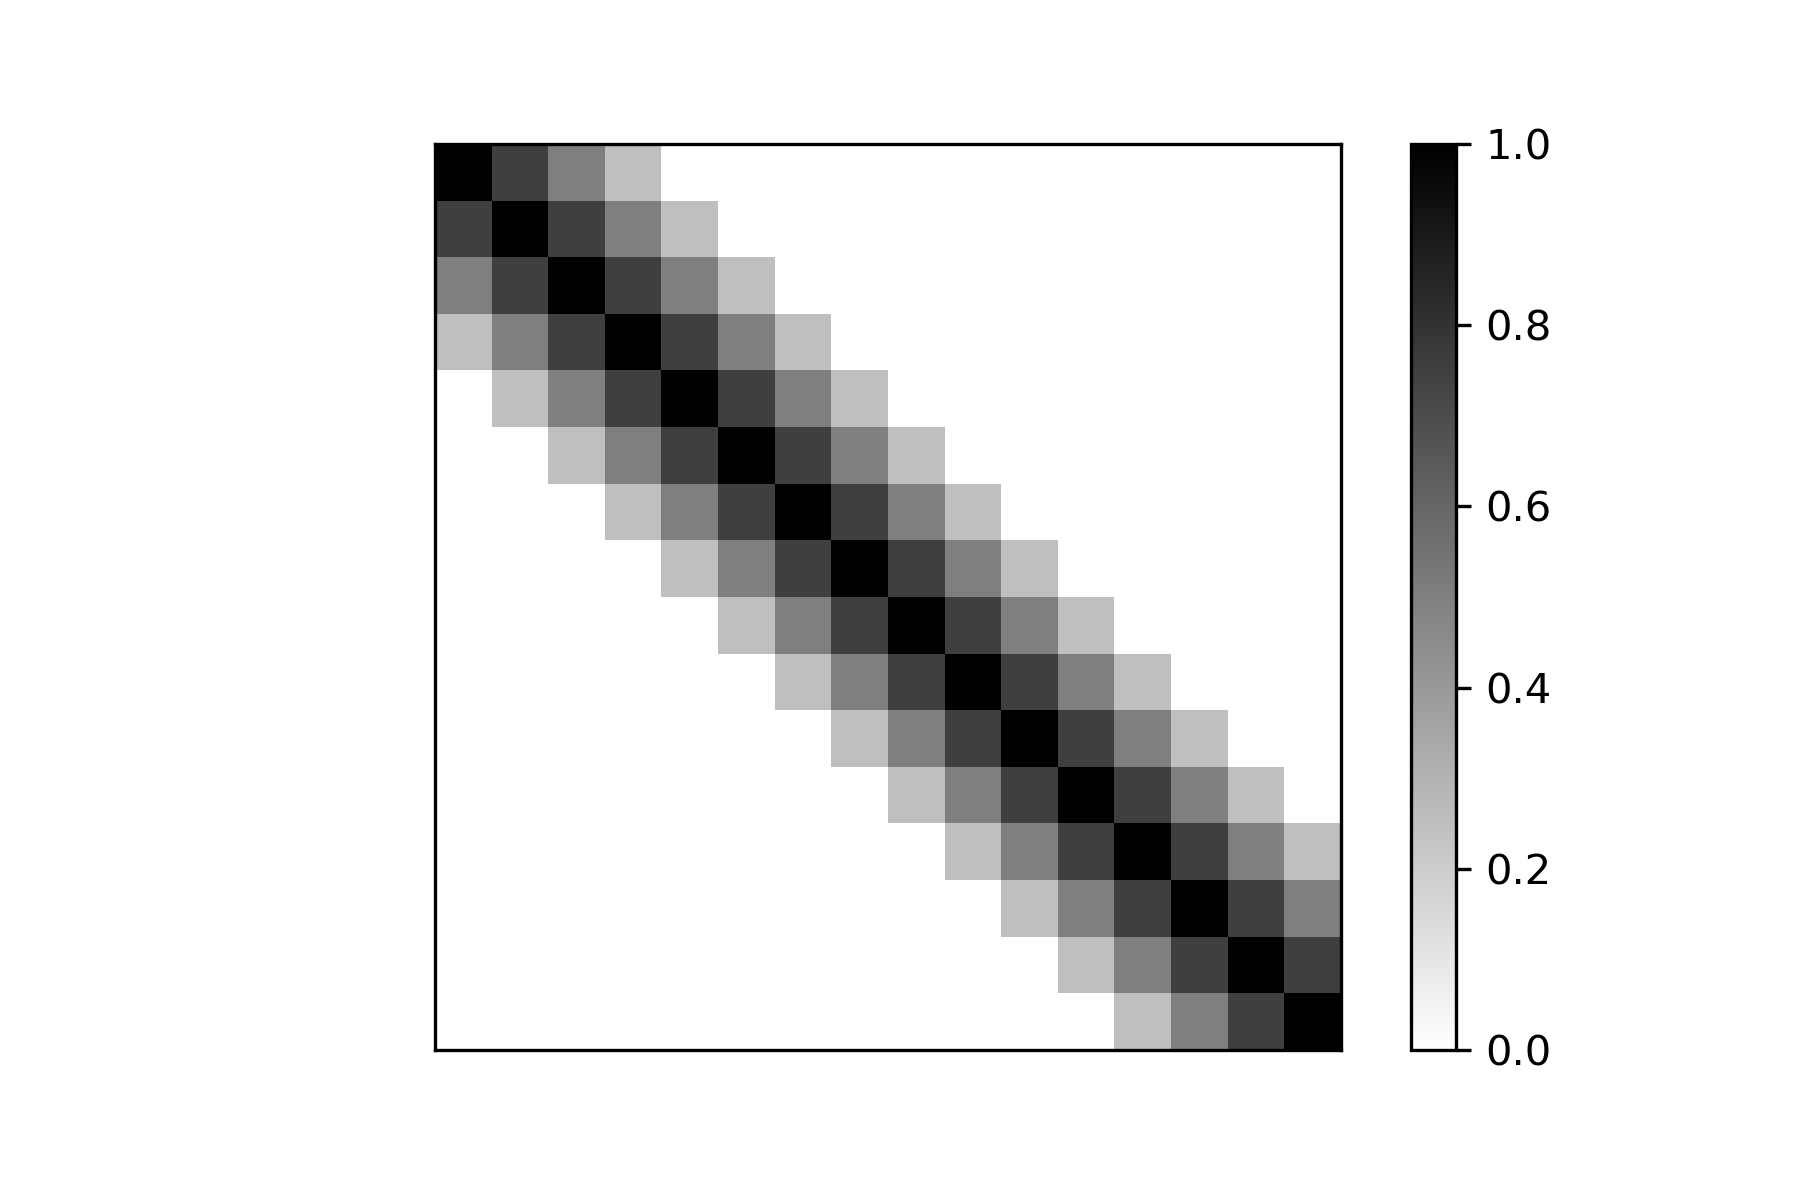
\includegraphics[width=4in]{03_04_img06.png}
\end{center}
Compute the singular value decomposition and plot the singular values
\begin{center}
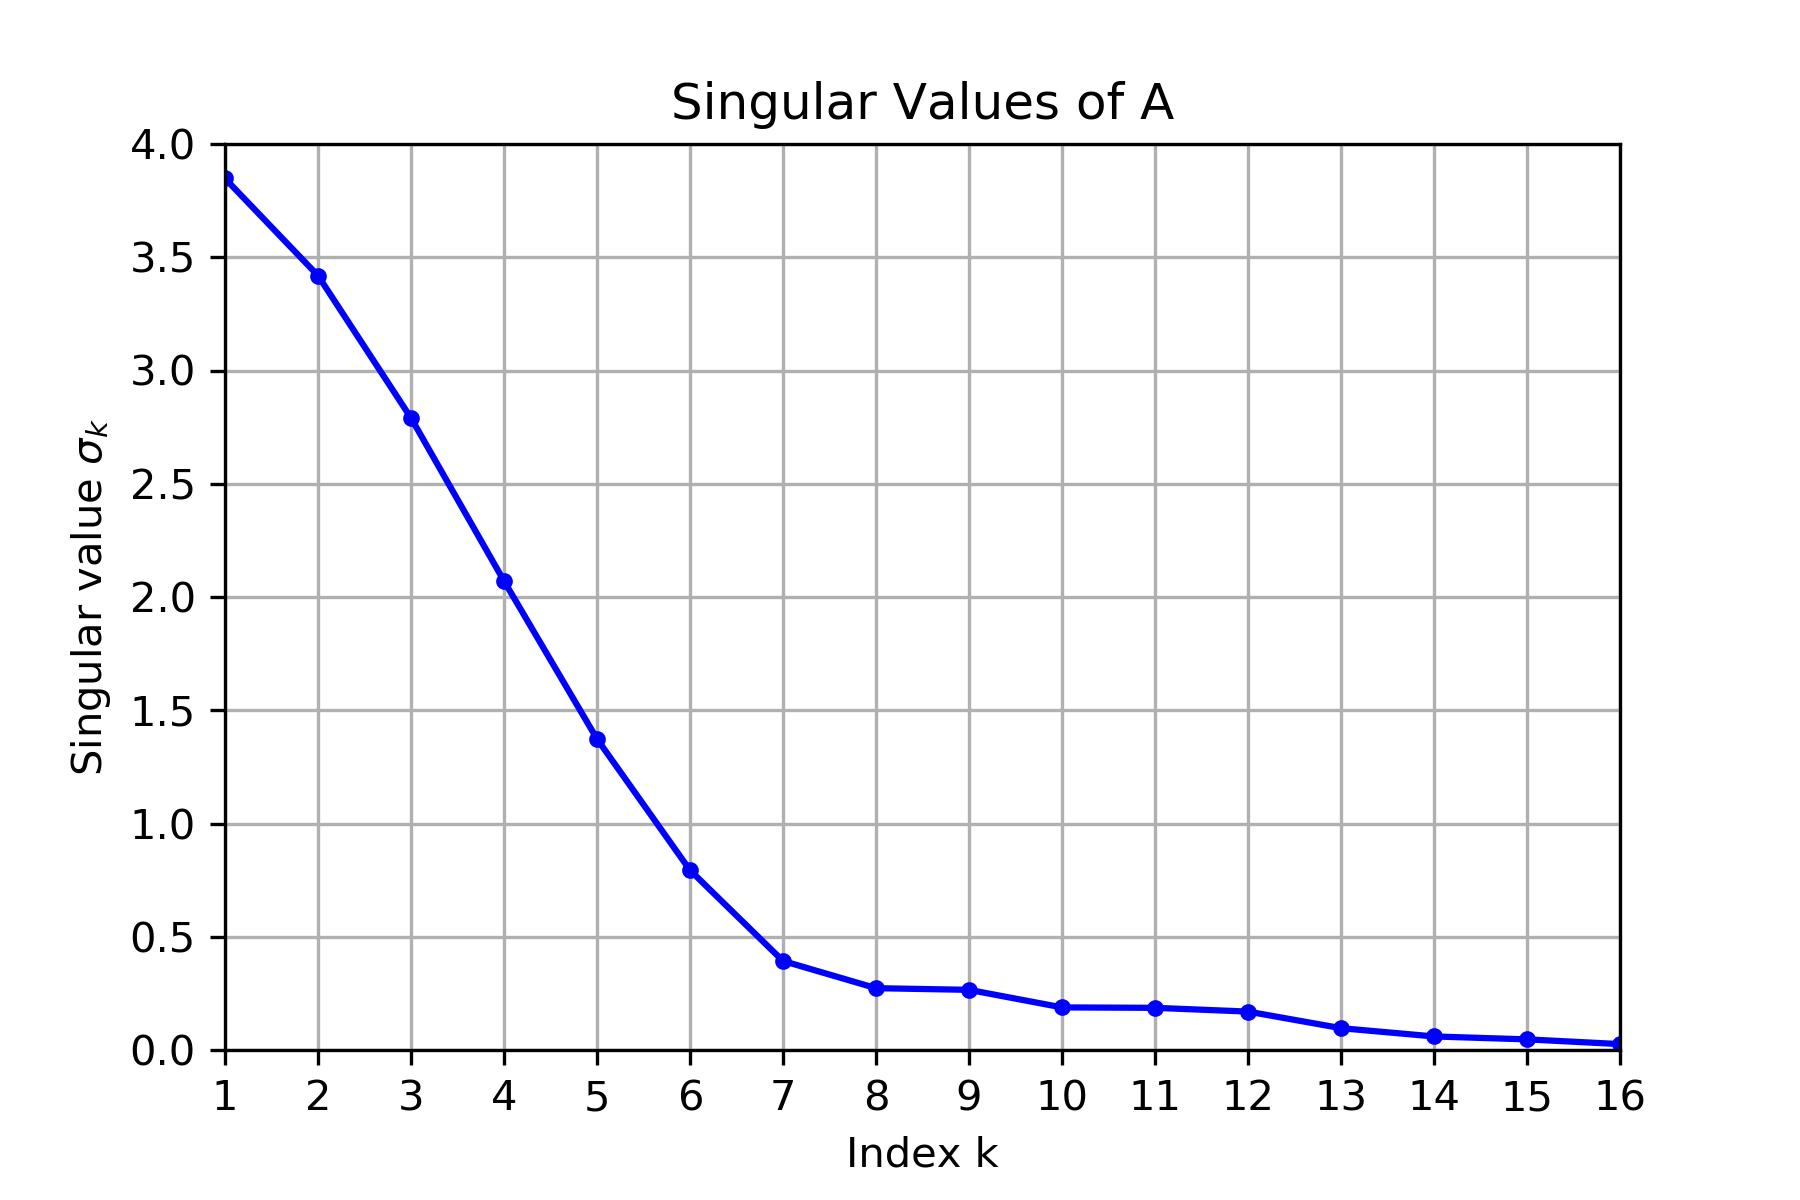
\includegraphics[width=4in]{03_04_img07.png}
\end{center}
For each $i=1,\dots,16$, plot the matrix $\sigma_i \bs{p}_i \bs{q}_i^T$:
\begin{center}
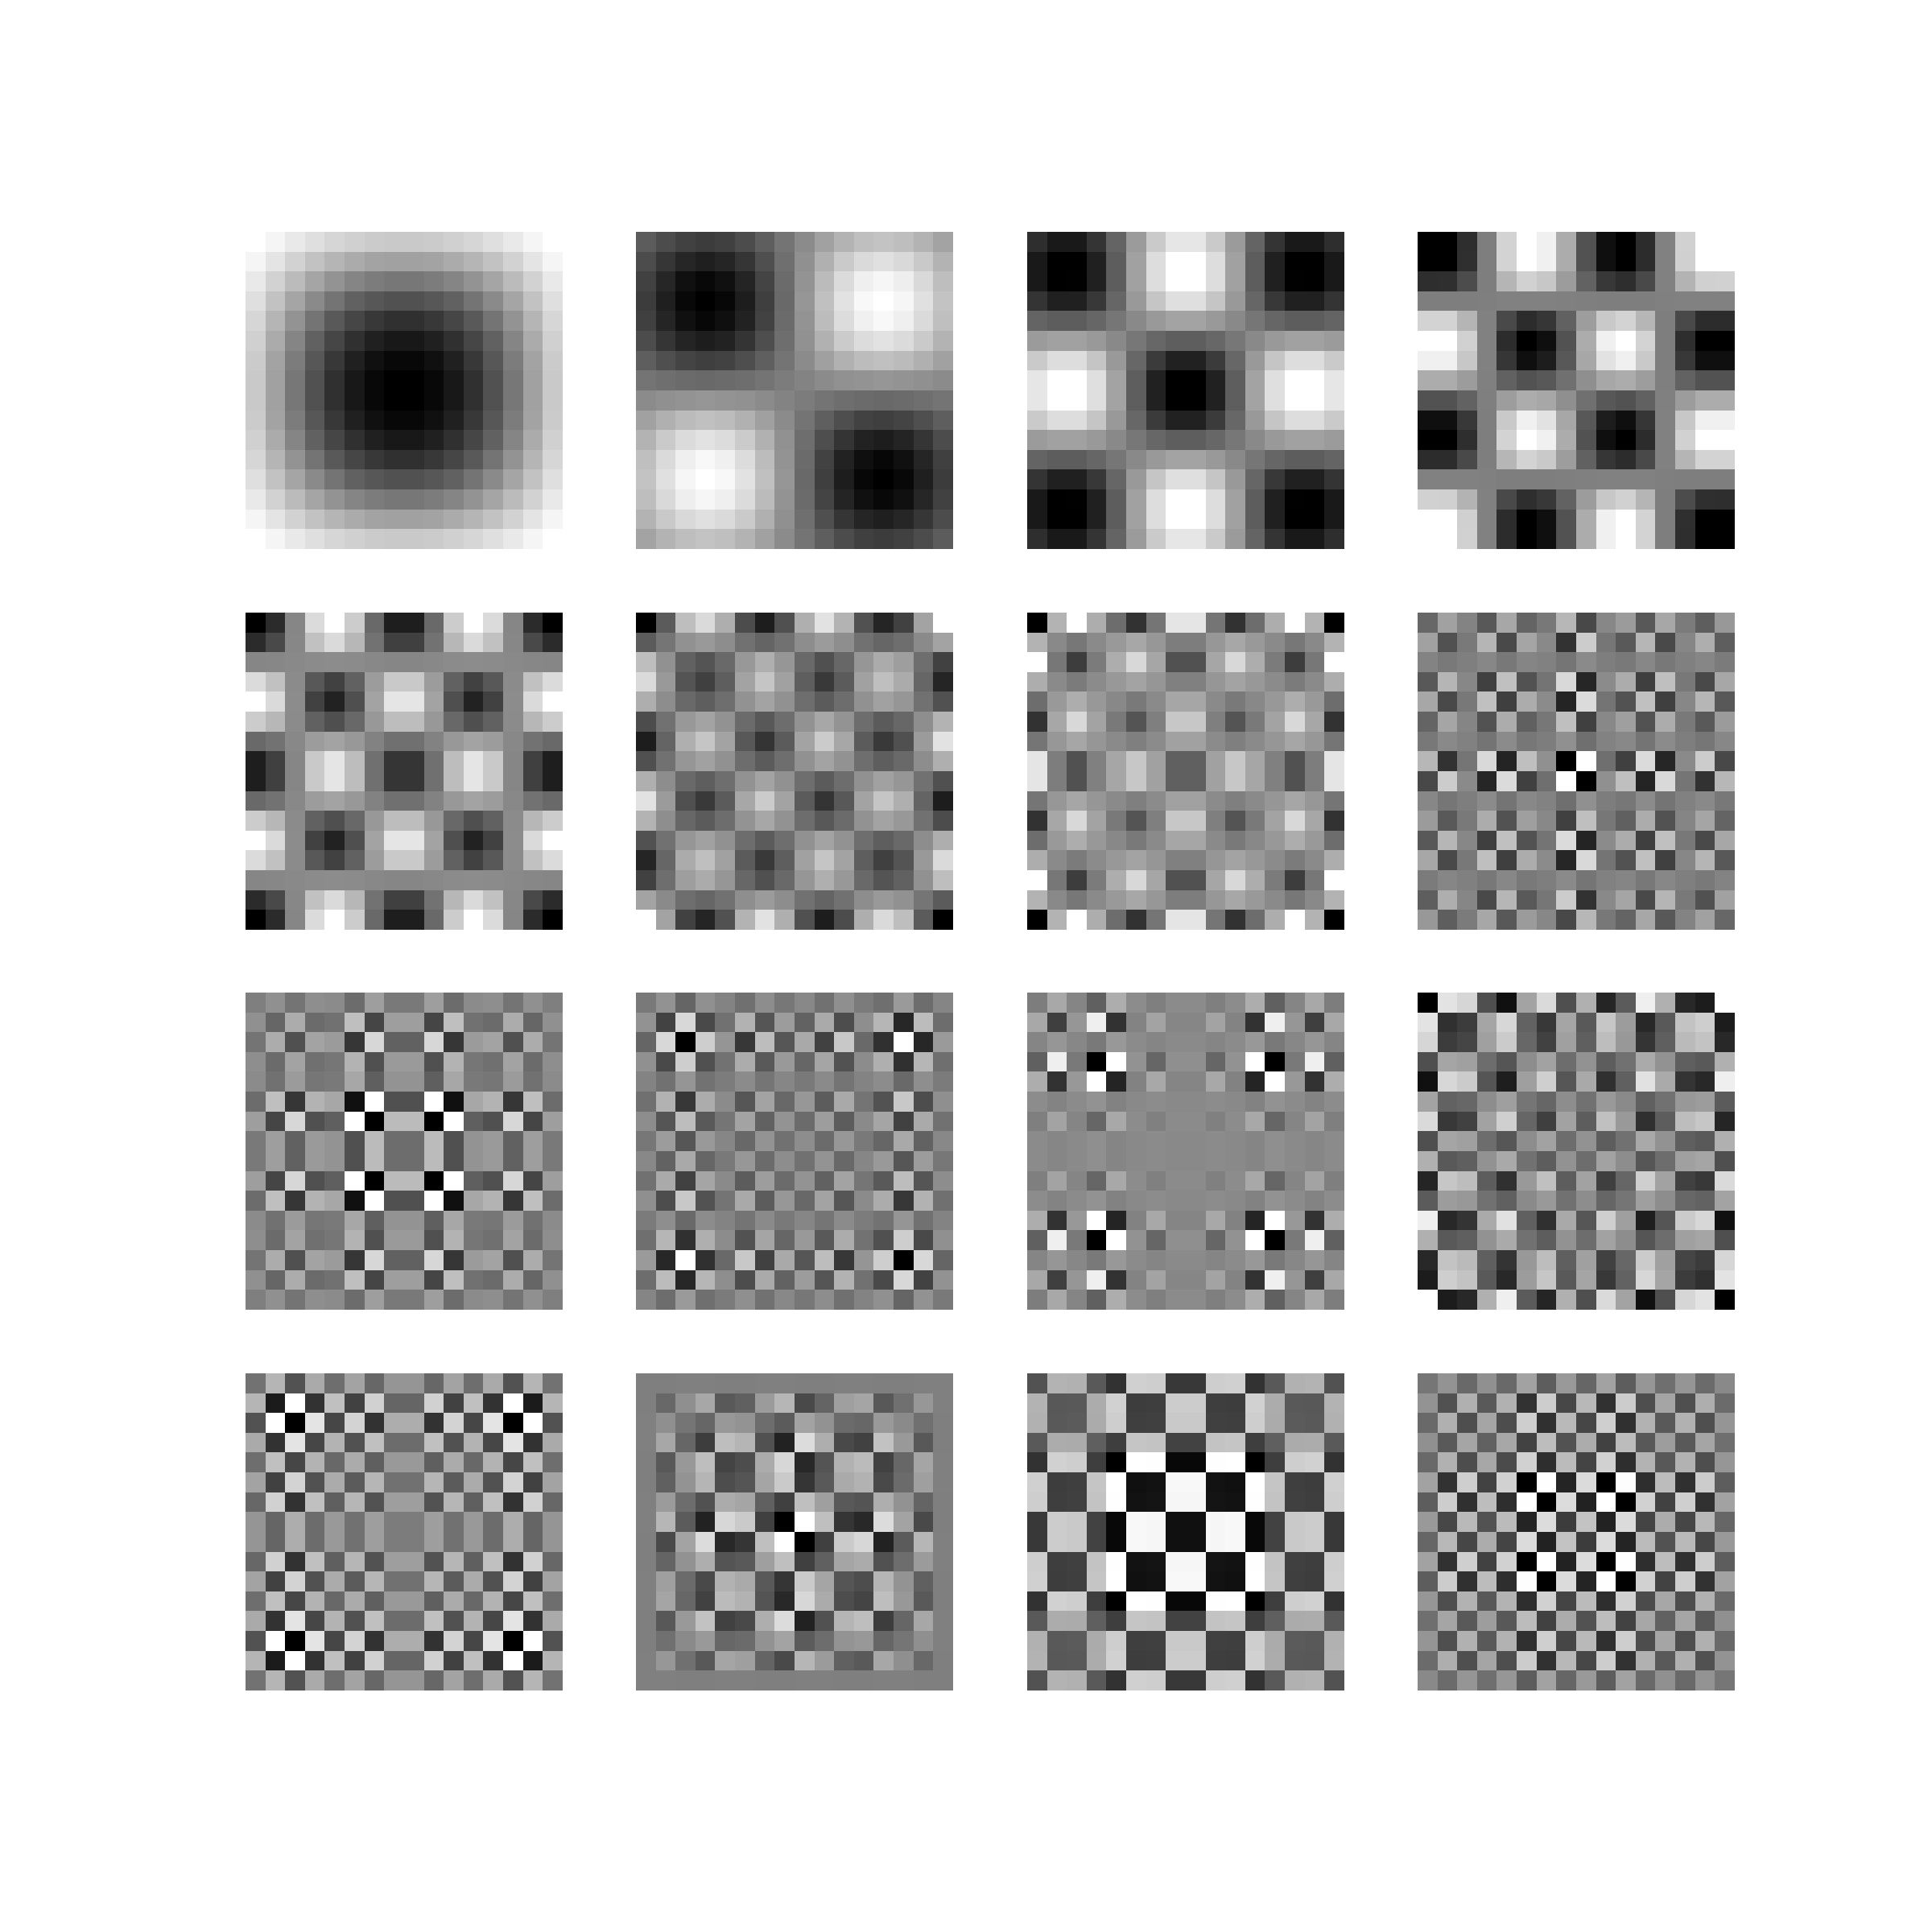
\includegraphics[width=3.5in]{03_04_img08.png}
\end{center}
For each $k=1,\dots,16$, plot the truncated SVD expansion of rank $k$
$$
A_k = \sum_{i=1}^k \sigma_i \bs{p}_i \bs{q}_i^T
$$
\begin{center}

\includegraphics[width=3.5in]{03_04_img09.png}
\end{center}
This shows that $A_k$ is very close to $A$ for $k \geq 12$ and therefore we can (and will) drop the smallest singular values of $A$ to compute the truncated pseudoinverse:
$$
A_k^+ = \sum_{i=1}^k \frac{1}{\sigma_i} \bs{q}_i \bs{p}_i^T
$$
\end{example}

\begin{example}
Consider the symmetric Toeplitz matrix $A$ from the previous example, and consider an image matrix $X$ with a block of 1s in the center:
\begin{center}

\includegraphics[width=4in]{03_04_img10.png}
\end{center}
Apply $A$ to both sides and denote the blurred image as $B$
$$
AXA^T = B
$$
Now suppose we add some random error $E$ to the blurred image
\begin{center}
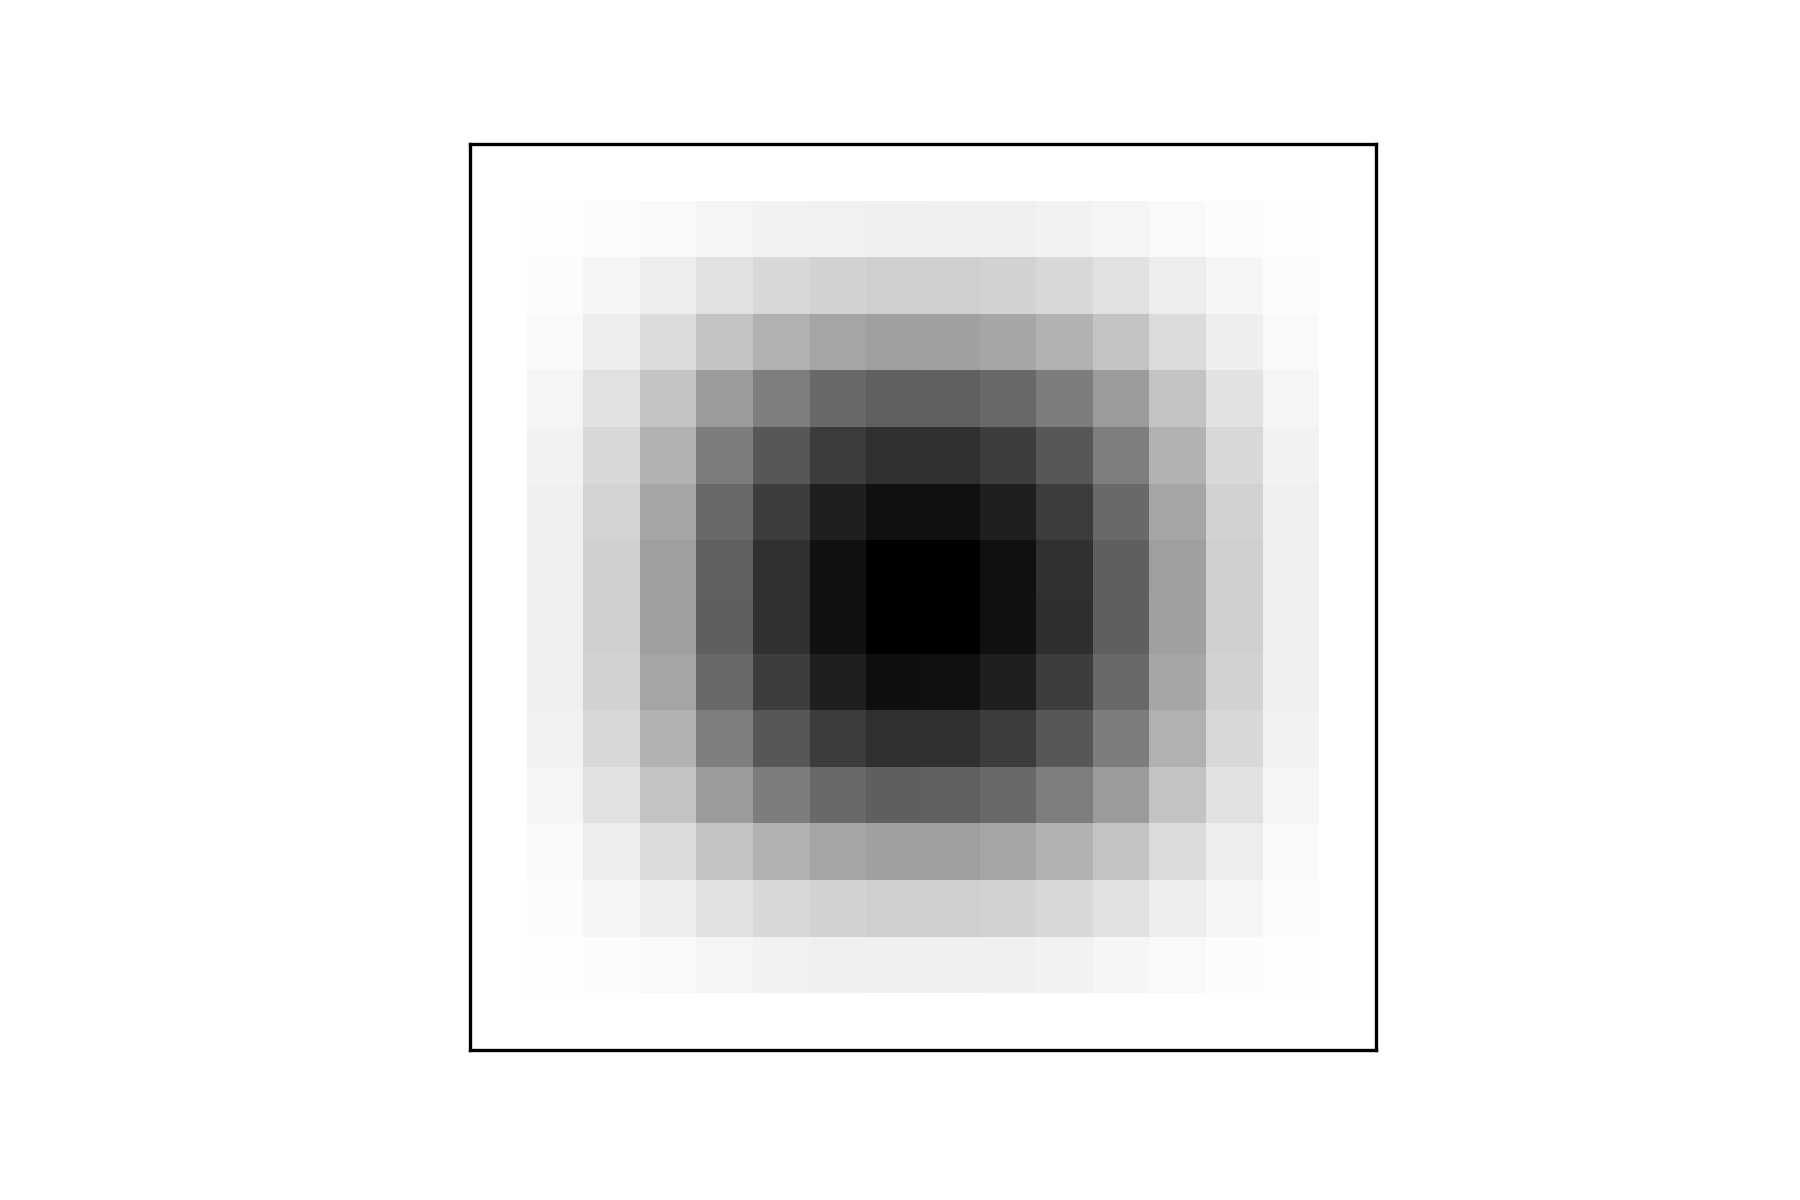
\includegraphics[width=4in]{03_04_img11.png}
\end{center}
We want to recover the original image by solving the equation
$$
A\hat{X}A^T = B + E
$$
If we solve the equation directly we get the image plus the inverted error
$$
\hat{X} = A^{-1}( B + E )(A^T)^{-1} = X + A^{-1} E (A^T)^{-1}
$$
\begin{center}
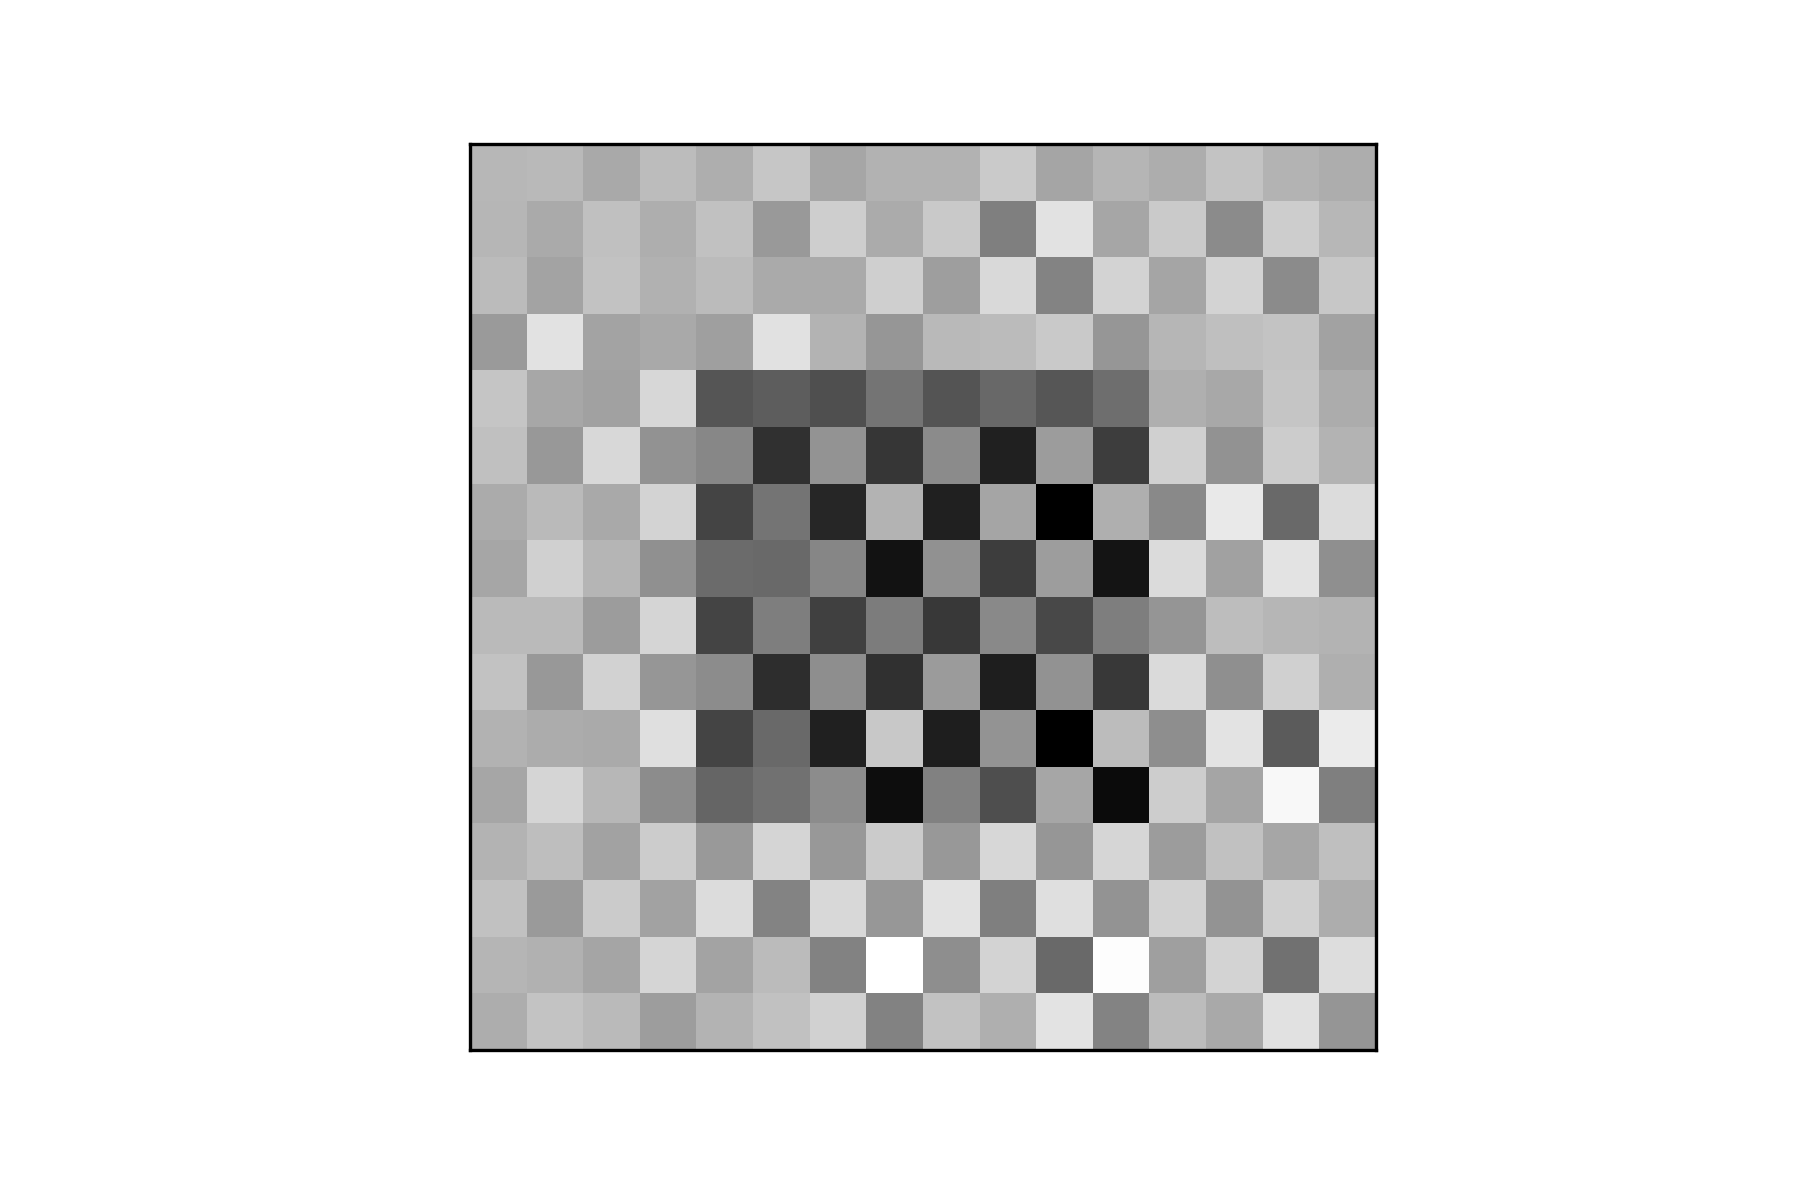
\includegraphics[width=4in]{03_04_img12.png}
\end{center}
In the previous example, we found that $A$ can be approximated by $A_k$ therefore we form the truncated pseudoinverse
$$
A_k^+ = \sum_{i=1}^k \frac{1}{\sigma_i} \bs{q}_i \bs{p}_i^T
$$
and compute for $k=12$
$$
\hat{X} = A_k^+(B +  E) (A^T)_k^+ = A_k^+B(A^T)_k^+ + A_k^+ E (A^T)_k^+
$$
\begin{center}
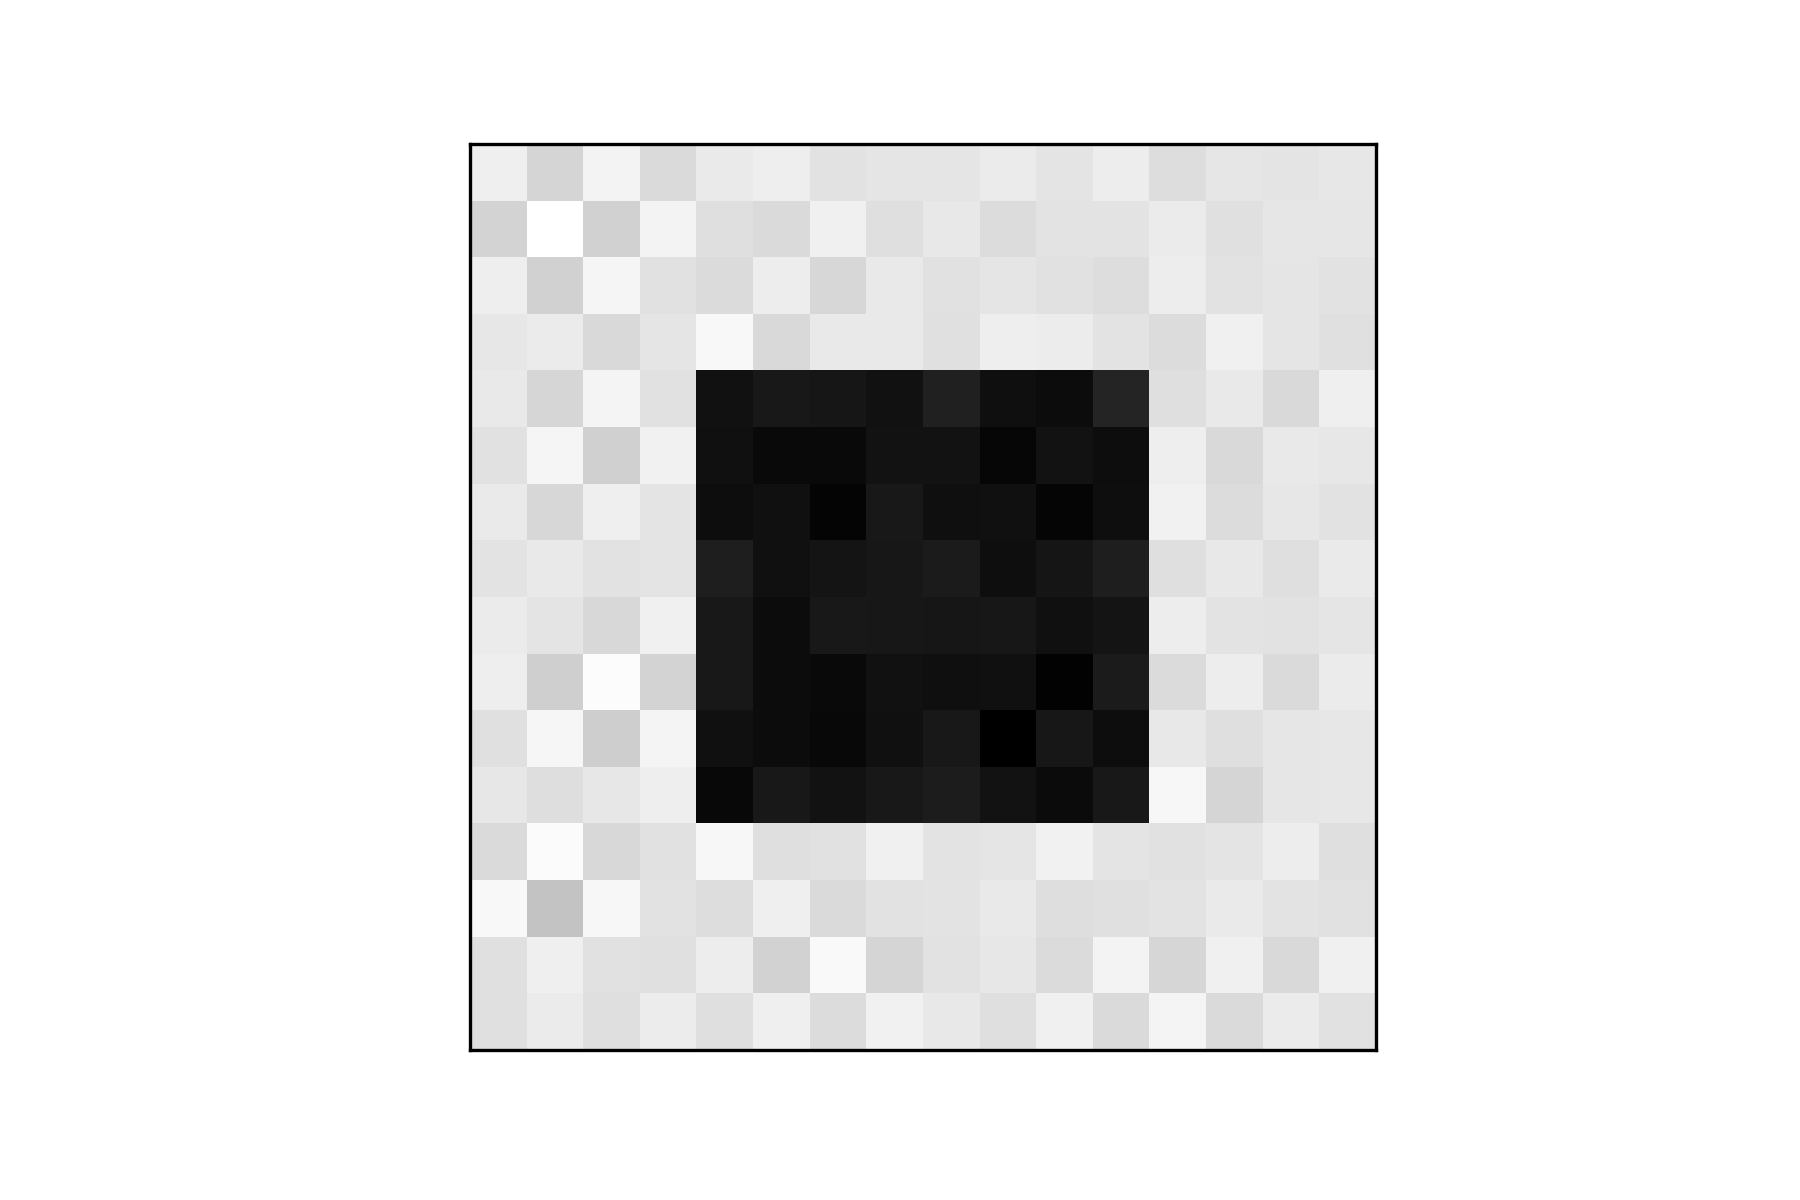
\includegraphics[width=4in]{03_04_img13.png}
\end{center}
The result is much better because the inverted error term $A_k^+ E (A^T)_k^+$ is smaller and so we avoid inverting too much of the error with small singular values.
\end{example}

